% Created by tikzDevice version 0.10.1 on 2016-11-21 07:40:35
% !TEX encoding = UTF-8 Unicode
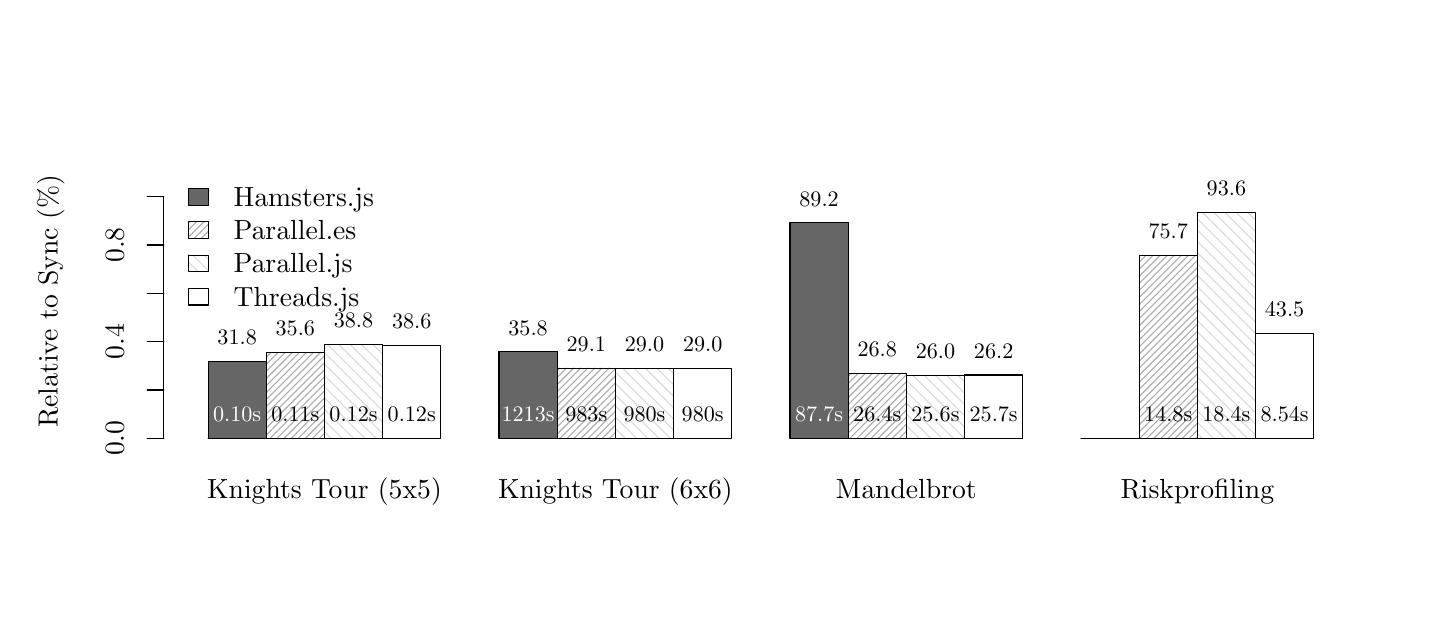
\begin{tikzpicture}[x=1pt,y=1pt]
\definecolor{fillColor}{RGB}{255,255,255}
\path[use as bounding box,fill=fillColor,fill opacity=0.00] (0,0) rectangle (505.89,209.58);
\begin{scope}
\path[clip] (  0.00,  0.00) rectangle (505.89,209.58);
\definecolor{fillColor}{gray}{0.40}

\path[fill=fillColor] ( 65.18, 61.20) --
	( 86.21, 61.20) --
	( 86.21, 88.94) --
	( 65.18, 88.94) --
	cycle;
\definecolor{drawColor}{RGB}{172,172,172}

\path[draw=drawColor,line width= 0.4pt,line join=round,line cap=round] ( 86.21, 90.48) -- ( 88.02, 92.29);

\path[draw=drawColor,line width= 0.4pt,line join=round,line cap=round] ( 86.21, 87.92) -- ( 90.58, 92.29);

\path[draw=drawColor,line width= 0.4pt,line join=round,line cap=round] ( 86.21, 85.37) -- ( 93.13, 92.29);

\path[draw=drawColor,line width= 0.4pt,line join=round,line cap=round] ( 86.21, 82.81) -- ( 95.69, 92.29);

\path[draw=drawColor,line width= 0.4pt,line join=round,line cap=round] ( 86.21, 80.26) -- ( 98.24, 92.29);

\path[draw=drawColor,line width= 0.4pt,line join=round,line cap=round] ( 86.21, 77.70) -- (100.80, 92.29);

\path[draw=drawColor,line width= 0.4pt,line join=round,line cap=round] ( 86.21, 75.15) -- (103.35, 92.29);

\path[draw=drawColor,line width= 0.4pt,line join=round,line cap=round] ( 86.21, 72.59) -- (105.91, 92.29);

\path[draw=drawColor,line width= 0.4pt,line join=round,line cap=round] ( 86.21, 70.04) -- (107.24, 91.07);

\path[draw=drawColor,line width= 0.4pt,line join=round,line cap=round] ( 86.21, 67.48) -- (107.24, 88.51);

\path[draw=drawColor,line width= 0.4pt,line join=round,line cap=round] ( 86.21, 64.93) -- (107.24, 85.96);

\path[draw=drawColor,line width= 0.4pt,line join=round,line cap=round] ( 86.21, 62.37) -- (107.24, 83.40);

\path[draw=drawColor,line width= 0.4pt,line join=round,line cap=round] ( 87.59, 61.20) -- (107.24, 80.85);

\path[draw=drawColor,line width= 0.4pt,line join=round,line cap=round] ( 90.15, 61.20) -- (107.24, 78.29);

\path[draw=drawColor,line width= 0.4pt,line join=round,line cap=round] ( 92.70, 61.20) -- (107.24, 75.74);

\path[draw=drawColor,line width= 0.4pt,line join=round,line cap=round] ( 95.26, 61.20) -- (107.24, 73.18);

\path[draw=drawColor,line width= 0.4pt,line join=round,line cap=round] ( 97.81, 61.20) -- (107.24, 70.63);

\path[draw=drawColor,line width= 0.4pt,line join=round,line cap=round] (100.37, 61.20) -- (107.24, 68.07);

\path[draw=drawColor,line width= 0.4pt,line join=round,line cap=round] (102.92, 61.20) -- (107.24, 65.52);

\path[draw=drawColor,line width= 0.4pt,line join=round,line cap=round] (105.48, 61.20) -- (107.24, 62.96);
\definecolor{drawColor}{RGB}{218,218,218}

\path[draw=drawColor,line width= 0.4pt,line join=round,line cap=round] (109.56, 61.20) -- (107.24, 63.53);

\path[draw=drawColor,line width= 0.4pt,line join=round,line cap=round] (113.65, 61.20) -- (107.24, 67.62);

\path[draw=drawColor,line width= 0.4pt,line join=round,line cap=round] (117.74, 61.20) -- (107.24, 71.70);

\path[draw=drawColor,line width= 0.4pt,line join=round,line cap=round] (121.83, 61.20) -- (107.24, 75.79);

\path[draw=drawColor,line width= 0.4pt,line join=round,line cap=round] (125.92, 61.20) -- (107.24, 79.88);

\path[draw=drawColor,line width= 0.4pt,line join=round,line cap=round] (128.26, 62.94) -- (107.24, 83.97);

\path[draw=drawColor,line width= 0.4pt,line join=round,line cap=round] (128.26, 67.03) -- (107.24, 88.06);

\path[draw=drawColor,line width= 0.4pt,line join=round,line cap=round] (128.26, 71.12) -- (107.24, 92.15);

\path[draw=drawColor,line width= 0.4pt,line join=round,line cap=round] (128.26, 75.21) -- (108.38, 95.10);

\path[draw=drawColor,line width= 0.4pt,line join=round,line cap=round] (128.26, 79.29) -- (112.46, 95.10);

\path[draw=drawColor,line width= 0.4pt,line join=round,line cap=round] (128.26, 83.38) -- (116.55, 95.10);

\path[draw=drawColor,line width= 0.4pt,line join=round,line cap=round] (128.26, 87.47) -- (120.64, 95.10);

\path[draw=drawColor,line width= 0.4pt,line join=round,line cap=round] (128.26, 91.56) -- (124.73, 95.10);

\path[fill=fillColor] (170.32, 61.20) --
	(191.35, 61.20) --
	(191.35, 92.49) --
	(170.32, 92.49) --
	cycle;
\definecolor{drawColor}{RGB}{172,172,172}

\path[draw=drawColor,line width= 0.4pt,line join=round,line cap=round] (191.35, 85.75) -- (192.17, 86.57);

\path[draw=drawColor,line width= 0.4pt,line join=round,line cap=round] (191.35, 83.19) -- (194.72, 86.57);

\path[draw=drawColor,line width= 0.4pt,line join=round,line cap=round] (191.35, 80.64) -- (197.28, 86.57);

\path[draw=drawColor,line width= 0.4pt,line join=round,line cap=round] (191.35, 78.08) -- (199.83, 86.57);

\path[draw=drawColor,line width= 0.4pt,line join=round,line cap=round] (191.35, 75.53) -- (202.39, 86.57);

\path[draw=drawColor,line width= 0.4pt,line join=round,line cap=round] (191.35, 72.97) -- (204.94, 86.57);

\path[draw=drawColor,line width= 0.4pt,line join=round,line cap=round] (191.35, 70.42) -- (207.50, 86.57);

\path[draw=drawColor,line width= 0.4pt,line join=round,line cap=round] (191.35, 67.86) -- (210.05, 86.57);

\path[draw=drawColor,line width= 0.4pt,line join=round,line cap=round] (191.35, 65.31) -- (212.38, 86.33);

\path[draw=drawColor,line width= 0.4pt,line join=round,line cap=round] (191.35, 62.75) -- (212.38, 83.78);

\path[draw=drawColor,line width= 0.4pt,line join=round,line cap=round] (192.35, 61.20) -- (212.38, 81.22);

\path[draw=drawColor,line width= 0.4pt,line join=round,line cap=round] (194.91, 61.20) -- (212.38, 78.67);

\path[draw=drawColor,line width= 0.4pt,line join=round,line cap=round] (197.46, 61.20) -- (212.38, 76.11);

\path[draw=drawColor,line width= 0.4pt,line join=round,line cap=round] (200.02, 61.20) -- (212.38, 73.56);

\path[draw=drawColor,line width= 0.4pt,line join=round,line cap=round] (202.57, 61.20) -- (212.38, 71.00);

\path[draw=drawColor,line width= 0.4pt,line join=round,line cap=round] (205.13, 61.20) -- (212.38, 68.45);

\path[draw=drawColor,line width= 0.4pt,line join=round,line cap=round] (207.68, 61.20) -- (212.38, 65.89);

\path[draw=drawColor,line width= 0.4pt,line join=round,line cap=round] (210.24, 61.20) -- (212.38, 63.34);
\definecolor{drawColor}{RGB}{218,218,218}

\path[draw=drawColor,line width= 0.4pt,line join=round,line cap=round] (215.86, 61.20) -- (212.38, 64.68);

\path[draw=drawColor,line width= 0.4pt,line join=round,line cap=round] (219.95, 61.20) -- (212.38, 68.77);

\path[draw=drawColor,line width= 0.4pt,line join=round,line cap=round] (224.03, 61.20) -- (212.38, 72.86);

\path[draw=drawColor,line width= 0.4pt,line join=round,line cap=round] (228.12, 61.20) -- (212.38, 76.95);

\path[draw=drawColor,line width= 0.4pt,line join=round,line cap=round] (232.21, 61.20) -- (212.38, 81.04);

\path[draw=drawColor,line width= 0.4pt,line join=round,line cap=round] (233.40, 64.10) -- (212.38, 85.12);

\path[draw=drawColor,line width= 0.4pt,line join=round,line cap=round] (233.40, 68.18) -- (215.09, 86.50);

\path[draw=drawColor,line width= 0.4pt,line join=round,line cap=round] (233.40, 72.27) -- (219.18, 86.50);

\path[draw=drawColor,line width= 0.4pt,line join=round,line cap=round] (233.40, 76.36) -- (223.27, 86.50);

\path[draw=drawColor,line width= 0.4pt,line join=round,line cap=round] (233.40, 80.45) -- (227.36, 86.50);

\path[draw=drawColor,line width= 0.4pt,line join=round,line cap=round] (233.40, 84.54) -- (231.45, 86.50);

\path[fill=fillColor] (275.46, 61.20) --
	(296.49, 61.20) --
	(296.49,139.11) --
	(275.46,139.11) --
	cycle;
\definecolor{drawColor}{RGB}{172,172,172}

\path[draw=drawColor,line width= 0.4pt,line join=round,line cap=round] (296.49, 83.57) -- (297.54, 84.62);

\path[draw=drawColor,line width= 0.4pt,line join=round,line cap=round] (296.49, 81.02) -- (300.09, 84.62);

\path[draw=drawColor,line width= 0.4pt,line join=round,line cap=round] (296.49, 78.46) -- (302.65, 84.62);

\path[draw=drawColor,line width= 0.4pt,line join=round,line cap=round] (296.49, 75.91) -- (305.20, 84.62);

\path[draw=drawColor,line width= 0.4pt,line join=round,line cap=round] (296.49, 73.35) -- (307.76, 84.62);

\path[draw=drawColor,line width= 0.4pt,line join=round,line cap=round] (296.49, 70.80) -- (310.31, 84.62);

\path[draw=drawColor,line width= 0.4pt,line join=round,line cap=round] (296.49, 68.24) -- (312.87, 84.62);

\path[draw=drawColor,line width= 0.4pt,line join=round,line cap=round] (296.49, 65.69) -- (315.42, 84.62);

\path[draw=drawColor,line width= 0.4pt,line join=round,line cap=round] (296.49, 63.13) -- (317.51, 84.16);

\path[draw=drawColor,line width= 0.4pt,line join=round,line cap=round] (297.11, 61.20) -- (317.51, 81.60);

\path[draw=drawColor,line width= 0.4pt,line join=round,line cap=round] (299.67, 61.20) -- (317.51, 79.05);

\path[draw=drawColor,line width= 0.4pt,line join=round,line cap=round] (302.22, 61.20) -- (317.51, 76.49);

\path[draw=drawColor,line width= 0.4pt,line join=round,line cap=round] (304.78, 61.20) -- (317.51, 73.94);

\path[draw=drawColor,line width= 0.4pt,line join=round,line cap=round] (307.33, 61.20) -- (317.51, 71.38);

\path[draw=drawColor,line width= 0.4pt,line join=round,line cap=round] (309.89, 61.20) -- (317.51, 68.83);

\path[draw=drawColor,line width= 0.4pt,line join=round,line cap=round] (312.44, 61.20) -- (317.51, 66.27);

\path[draw=drawColor,line width= 0.4pt,line join=round,line cap=round] (315.00, 61.20) -- (317.51, 63.72);
\definecolor{drawColor}{RGB}{218,218,218}

\path[draw=drawColor,line width= 0.4pt,line join=round,line cap=round] (318.06, 61.20) -- (317.51, 61.75);

\path[draw=drawColor,line width= 0.4pt,line join=round,line cap=round] (322.15, 61.20) -- (317.51, 65.84);

\path[draw=drawColor,line width= 0.4pt,line join=round,line cap=round] (326.24, 61.20) -- (317.51, 69.93);

\path[draw=drawColor,line width= 0.4pt,line join=round,line cap=round] (330.33, 61.20) -- (317.51, 74.01);

\path[draw=drawColor,line width= 0.4pt,line join=round,line cap=round] (334.42, 61.20) -- (317.51, 78.10);

\path[draw=drawColor,line width= 0.4pt,line join=round,line cap=round] (338.50, 61.20) -- (317.51, 82.19);

\path[draw=drawColor,line width= 0.4pt,line join=round,line cap=round] (338.54, 65.25) -- (319.88, 83.91);

\path[draw=drawColor,line width= 0.4pt,line join=round,line cap=round] (338.54, 69.34) -- (323.97, 83.91);

\path[draw=drawColor,line width= 0.4pt,line join=round,line cap=round] (338.54, 73.43) -- (328.06, 83.91);

\path[draw=drawColor,line width= 0.4pt,line join=round,line cap=round] (338.54, 77.51) -- (332.15, 83.91);

\path[draw=drawColor,line width= 0.4pt,line join=round,line cap=round] (338.54, 81.60) -- (336.24, 83.91);

\path[fill=fillColor] (380.60, 61.20) --
	(401.63, 61.20) --
	cycle;
\definecolor{drawColor}{RGB}{172,172,172}

\path[draw=drawColor,line width= 0.4pt,line join=round,line cap=round] (401.63,124.83) -- (404.07,127.28);

\path[draw=drawColor,line width= 0.4pt,line join=round,line cap=round] (401.63,122.28) -- (406.63,127.28);

\path[draw=drawColor,line width= 0.4pt,line join=round,line cap=round] (401.63,119.72) -- (409.18,127.28);

\path[draw=drawColor,line width= 0.4pt,line join=round,line cap=round] (401.63,117.17) -- (411.74,127.28);

\path[draw=drawColor,line width= 0.4pt,line join=round,line cap=round] (401.63,114.61) -- (414.29,127.28);

\path[draw=drawColor,line width= 0.4pt,line join=round,line cap=round] (401.63,112.06) -- (416.85,127.28);

\path[draw=drawColor,line width= 0.4pt,line join=round,line cap=round] (401.63,109.50) -- (419.40,127.28);

\path[draw=drawColor,line width= 0.4pt,line join=round,line cap=round] (401.63,106.95) -- (421.96,127.28);

\path[draw=drawColor,line width= 0.4pt,line join=round,line cap=round] (401.63,104.39) -- (422.65,125.42);

\path[draw=drawColor,line width= 0.4pt,line join=round,line cap=round] (401.63,101.84) -- (422.65,122.86);

\path[draw=drawColor,line width= 0.4pt,line join=round,line cap=round] (401.63, 99.28) -- (422.65,120.31);

\path[draw=drawColor,line width= 0.4pt,line join=round,line cap=round] (401.63, 96.73) -- (422.65,117.75);

\path[draw=drawColor,line width= 0.4pt,line join=round,line cap=round] (401.63, 94.17) -- (422.65,115.20);

\path[draw=drawColor,line width= 0.4pt,line join=round,line cap=round] (401.63, 91.62) -- (422.65,112.64);

\path[draw=drawColor,line width= 0.4pt,line join=round,line cap=round] (401.63, 89.06) -- (422.65,110.09);

\path[draw=drawColor,line width= 0.4pt,line join=round,line cap=round] (401.63, 86.51) -- (422.65,107.53);

\path[draw=drawColor,line width= 0.4pt,line join=round,line cap=round] (401.63, 83.95) -- (422.65,104.98);

\path[draw=drawColor,line width= 0.4pt,line join=round,line cap=round] (401.63, 81.40) -- (422.65,102.42);

\path[draw=drawColor,line width= 0.4pt,line join=round,line cap=round] (401.63, 78.84) -- (422.65, 99.87);

\path[draw=drawColor,line width= 0.4pt,line join=round,line cap=round] (401.63, 76.28) -- (422.65, 97.31);

\path[draw=drawColor,line width= 0.4pt,line join=round,line cap=round] (401.63, 73.73) -- (422.65, 94.76);

\path[draw=drawColor,line width= 0.4pt,line join=round,line cap=round] (401.63, 71.17) -- (422.65, 92.20);

\path[draw=drawColor,line width= 0.4pt,line join=round,line cap=round] (401.63, 68.62) -- (422.65, 89.65);

\path[draw=drawColor,line width= 0.4pt,line join=round,line cap=round] (401.63, 66.06) -- (422.65, 87.09);

\path[draw=drawColor,line width= 0.4pt,line join=round,line cap=round] (401.63, 63.51) -- (422.65, 84.54);

\path[draw=drawColor,line width= 0.4pt,line join=round,line cap=round] (401.87, 61.20) -- (422.65, 81.98);

\path[draw=drawColor,line width= 0.4pt,line join=round,line cap=round] (404.43, 61.20) -- (422.65, 79.43);

\path[draw=drawColor,line width= 0.4pt,line join=round,line cap=round] (406.98, 61.20) -- (422.65, 76.87);

\path[draw=drawColor,line width= 0.4pt,line join=round,line cap=round] (409.54, 61.20) -- (422.65, 74.32);

\path[draw=drawColor,line width= 0.4pt,line join=round,line cap=round] (412.09, 61.20) -- (422.65, 71.76);

\path[draw=drawColor,line width= 0.4pt,line join=round,line cap=round] (414.65, 61.20) -- (422.65, 69.21);

\path[draw=drawColor,line width= 0.4pt,line join=round,line cap=round] (417.20, 61.20) -- (422.65, 66.65);

\path[draw=drawColor,line width= 0.4pt,line join=round,line cap=round] (419.76, 61.20) -- (422.65, 64.10);

\path[draw=drawColor,line width= 0.4pt,line join=round,line cap=round] (422.31, 61.20) -- (422.65, 61.54);
\definecolor{drawColor}{RGB}{218,218,218}

\path[draw=drawColor,line width= 0.4pt,line join=round,line cap=round] (424.36, 61.20) -- (422.65, 62.90);

\path[draw=drawColor,line width= 0.4pt,line join=round,line cap=round] (428.44, 61.20) -- (422.65, 66.99);

\path[draw=drawColor,line width= 0.4pt,line join=round,line cap=round] (432.53, 61.20) -- (422.65, 71.08);

\path[draw=drawColor,line width= 0.4pt,line join=round,line cap=round] (436.62, 61.20) -- (422.65, 75.17);

\path[draw=drawColor,line width= 0.4pt,line join=round,line cap=round] (440.71, 61.20) -- (422.65, 79.26);

\path[draw=drawColor,line width= 0.4pt,line join=round,line cap=round] (443.68, 62.32) -- (422.65, 83.34);

\path[draw=drawColor,line width= 0.4pt,line join=round,line cap=round] (443.68, 66.40) -- (422.65, 87.43);

\path[draw=drawColor,line width= 0.4pt,line join=round,line cap=round] (443.68, 70.49) -- (422.65, 91.52);

\path[draw=drawColor,line width= 0.4pt,line join=round,line cap=round] (443.68, 74.58) -- (422.65, 95.61);

\path[draw=drawColor,line width= 0.4pt,line join=round,line cap=round] (443.68, 78.67) -- (422.65, 99.70);

\path[draw=drawColor,line width= 0.4pt,line join=round,line cap=round] (443.68, 82.76) -- (422.65,103.79);

\path[draw=drawColor,line width= 0.4pt,line join=round,line cap=round] (443.68, 86.85) -- (422.65,107.87);

\path[draw=drawColor,line width= 0.4pt,line join=round,line cap=round] (443.68, 90.93) -- (422.65,111.96);

\path[draw=drawColor,line width= 0.4pt,line join=round,line cap=round] (443.68, 95.02) -- (422.65,116.05);

\path[draw=drawColor,line width= 0.4pt,line join=round,line cap=round] (443.68, 99.11) -- (422.65,120.14);

\path[draw=drawColor,line width= 0.4pt,line join=round,line cap=round] (443.68,103.20) -- (422.65,124.23);

\path[draw=drawColor,line width= 0.4pt,line join=round,line cap=round] (443.68,107.29) -- (422.65,128.31);

\path[draw=drawColor,line width= 0.4pt,line join=round,line cap=round] (443.68,111.38) -- (422.65,132.40);

\path[draw=drawColor,line width= 0.4pt,line join=round,line cap=round] (443.68,115.46) -- (422.65,136.49);

\path[draw=drawColor,line width= 0.4pt,line join=round,line cap=round] (443.68,119.55) -- (422.65,140.58);

\path[draw=drawColor,line width= 0.4pt,line join=round,line cap=round] (443.68,123.64) -- (424.40,142.92);

\path[draw=drawColor,line width= 0.4pt,line join=round,line cap=round] (443.68,127.73) -- (428.49,142.92);

\path[draw=drawColor,line width= 0.4pt,line join=round,line cap=round] (443.68,131.82) -- (432.58,142.92);

\path[draw=drawColor,line width= 0.4pt,line join=round,line cap=round] (443.68,135.90) -- (436.66,142.92);

\path[draw=drawColor,line width= 0.4pt,line join=round,line cap=round] (443.68,139.99) -- (440.75,142.92);
\definecolor{drawColor}{RGB}{0,0,0}

\path[draw=drawColor,line width= 0.4pt,line join=round,line cap=round] ( 65.18, 61.20) --
	( 86.21, 61.20) --
	( 86.21, 88.94) --
	( 65.18, 88.94) --
	( 65.18, 61.20);

\path[draw=drawColor,line width= 0.4pt,line join=round,line cap=round] ( 86.21, 61.20) --
	(107.24, 61.20) --
	(107.24, 92.29) --
	( 86.21, 92.29) --
	( 86.21, 61.20);

\path[draw=drawColor,line width= 0.4pt,line join=round,line cap=round] (107.24, 61.20) --
	(128.26, 61.20) --
	(128.26, 95.10) --
	(107.24, 95.10) --
	(107.24, 61.20);

\path[draw=drawColor,line width= 0.4pt,line join=round,line cap=round] (128.26, 61.20) --
	(149.29, 61.20) --
	(149.29, 94.88) --
	(128.26, 94.88) --
	(128.26, 61.20);

\path[draw=drawColor,line width= 0.4pt,line join=round,line cap=round] (170.32, 61.20) --
	(191.35, 61.20) --
	(191.35, 92.49) --
	(170.32, 92.49) --
	(170.32, 61.20);

\path[draw=drawColor,line width= 0.4pt,line join=round,line cap=round] (191.35, 61.20) --
	(212.38, 61.20) --
	(212.38, 86.57) --
	(191.35, 86.57) --
	(191.35, 61.20);

\path[draw=drawColor,line width= 0.4pt,line join=round,line cap=round] (212.38, 61.20) --
	(233.40, 61.20) --
	(233.40, 86.50) --
	(212.38, 86.50) --
	(212.38, 61.20);

\path[draw=drawColor,line width= 0.4pt,line join=round,line cap=round] (233.40, 61.20) --
	(254.43, 61.20) --
	(254.43, 86.48) --
	(233.40, 86.48) --
	(233.40, 61.20);

\path[draw=drawColor,line width= 0.4pt,line join=round,line cap=round] (275.46, 61.20) --
	(296.49, 61.20) --
	(296.49,139.11) --
	(275.46,139.11) --
	(275.46, 61.20);

\path[draw=drawColor,line width= 0.4pt,line join=round,line cap=round] (296.49, 61.20) --
	(317.51, 61.20) --
	(317.51, 84.62) --
	(296.49, 84.62) --
	(296.49, 61.20);

\path[draw=drawColor,line width= 0.4pt,line join=round,line cap=round] (317.51, 61.20) --
	(338.54, 61.20) --
	(338.54, 83.91) --
	(317.51, 83.91) --
	(317.51, 61.20);

\path[draw=drawColor,line width= 0.4pt,line join=round,line cap=round] (338.54, 61.20) --
	(359.57, 61.20) --
	(359.57, 84.07) --
	(338.54, 84.07) --
	(338.54, 61.20);

\path[draw=drawColor,line width= 0.4pt,line join=round,line cap=round] (380.60, 61.20) --
	(401.63, 61.20) --
	(380.60, 61.20);

\path[draw=drawColor,line width= 0.4pt,line join=round,line cap=round] (401.63, 61.20) --
	(422.65, 61.20) --
	(422.65,127.28) --
	(401.63,127.28) --
	(401.63, 61.20);

\path[draw=drawColor,line width= 0.4pt,line join=round,line cap=round] (422.65, 61.20) --
	(443.68, 61.20) --
	(443.68,142.92) --
	(422.65,142.92) --
	(422.65, 61.20);

\path[draw=drawColor,line width= 0.4pt,line join=round,line cap=round] (443.68, 61.20) --
	(464.71, 61.20) --
	(464.71, 99.21) --
	(443.68, 99.21) --
	(443.68, 61.20);
\end{scope}
\begin{scope}
\path[clip] (  0.00,  0.00) rectangle (505.89,209.58);
\definecolor{drawColor}{RGB}{0,0,0}

\node[text=drawColor,anchor=base,inner sep=0pt, outer sep=0pt, scale=  1.00] at (107.24, 39.60) {Knights Tour (5x5)};

\node[text=drawColor,anchor=base,inner sep=0pt, outer sep=0pt, scale=  1.00] at (212.38, 39.60) {Knights Tour (6x6)};

\node[text=drawColor,anchor=base,inner sep=0pt, outer sep=0pt, scale=  1.00] at (317.51, 39.60) {Mandelbrot};

\node[text=drawColor,anchor=base,inner sep=0pt, outer sep=0pt, scale=  1.00] at (422.65, 39.60) {Riskprofiling};
\end{scope}
\begin{scope}
\path[clip] (  0.00,  0.00) rectangle (505.89,209.58);
\definecolor{drawColor}{RGB}{0,0,0}

\node[text=drawColor,rotate= 90.00,anchor=base,inner sep=0pt, outer sep=0pt, scale=  1.00] at ( 10.80,110.79) {Relative to Sync ({\%})};
\end{scope}
\begin{scope}
\path[clip] (  0.00,  0.00) rectangle (505.89,209.58);
\definecolor{drawColor}{RGB}{0,0,0}

\path[draw=drawColor,line width= 0.4pt,line join=round,line cap=round] ( 49.20, 61.20) -- ( 49.20,148.51);

\path[draw=drawColor,line width= 0.4pt,line join=round,line cap=round] ( 49.20, 61.20) -- ( 43.20, 61.20);

\path[draw=drawColor,line width= 0.4pt,line join=round,line cap=round] ( 49.20, 78.66) -- ( 43.20, 78.66);

\path[draw=drawColor,line width= 0.4pt,line join=round,line cap=round] ( 49.20, 96.12) -- ( 43.20, 96.12);

\path[draw=drawColor,line width= 0.4pt,line join=round,line cap=round] ( 49.20,113.58) -- ( 43.20,113.58);

\path[draw=drawColor,line width= 0.4pt,line join=round,line cap=round] ( 49.20,131.05) -- ( 43.20,131.05);

\path[draw=drawColor,line width= 0.4pt,line join=round,line cap=round] ( 49.20,148.51) -- ( 43.20,148.51);

\node[text=drawColor,rotate= 90.00,anchor=base,inner sep=0pt, outer sep=0pt, scale=  1.00] at ( 34.80, 61.20) {0.0};

\node[text=drawColor,rotate= 90.00,anchor=base,inner sep=0pt, outer sep=0pt, scale=  1.00] at ( 34.80, 96.12) {0.4};

\node[text=drawColor,rotate= 90.00,anchor=base,inner sep=0pt, outer sep=0pt, scale=  1.00] at ( 34.80,131.05) {0.8};
\end{scope}
\begin{scope}
\path[clip] ( 49.20, 61.20) rectangle (480.69,160.38);
\definecolor{fillColor}{gray}{0.40}

\path[fill=fillColor] ( 58.20,151.38) --
	( 65.40,151.38) --
	( 65.40,145.38) --
	( 58.20,145.38) --
	cycle;
\definecolor{drawColor}{RGB}{172,172,172}

\path[draw=drawColor,line width= 0.4pt,line join=round,line cap=round] ( 58.20,139.12) -- ( 58.46,139.38);

\path[draw=drawColor,line width= 0.4pt,line join=round,line cap=round] ( 58.20,136.57) -- ( 61.01,139.38);

\path[draw=drawColor,line width= 0.4pt,line join=round,line cap=round] ( 58.20,134.01) -- ( 63.57,139.38);

\path[draw=drawColor,line width= 0.4pt,line join=round,line cap=round] ( 60.12,133.38) -- ( 65.40,138.66);

\path[draw=drawColor,line width= 0.4pt,line join=round,line cap=round] ( 62.68,133.38) -- ( 65.40,136.10);

\path[draw=drawColor,line width= 0.4pt,line join=round,line cap=round] ( 65.23,133.38) -- ( 65.40,133.55);
\definecolor{drawColor}{RGB}{218,218,218}

\path[draw=drawColor,line width= 0.4pt,line join=round,line cap=round] ( 61.65,121.38) -- ( 58.20,124.83);

\path[draw=drawColor,line width= 0.4pt,line join=round,line cap=round] ( 65.40,121.72) -- ( 59.73,127.38);

\path[draw=drawColor,line width= 0.4pt,line join=round,line cap=round] ( 65.40,125.81) -- ( 63.82,127.38);
\definecolor{drawColor}{RGB}{0,0,0}

\path[draw=drawColor,line width= 0.4pt,line join=round,line cap=round] ( 58.20,151.38) --
	( 65.40,151.38) --
	( 65.40,145.38) --
	( 58.20,145.38) --
	( 58.20,151.38);

\path[draw=drawColor,line width= 0.4pt,line join=round,line cap=round] ( 58.20,139.38) --
	( 65.40,139.38) --
	( 65.40,133.38) --
	( 58.20,133.38) --
	( 58.20,139.38);

\path[draw=drawColor,line width= 0.4pt,line join=round,line cap=round] ( 58.20,127.38) --
	( 65.40,127.38) --
	( 65.40,121.38) --
	( 58.20,121.38) --
	( 58.20,127.38);

\path[draw=drawColor,line width= 0.4pt,line join=round,line cap=round] ( 58.20,115.38) --
	( 65.40,115.38) --
	( 65.40,109.38) --
	( 58.20,109.38) --
	( 58.20,115.38);

\node[text=drawColor,anchor=base west,inner sep=0pt, outer sep=0pt, scale=  1.00] at ( 74.40,144.94) {Hamsters.js};

\node[text=drawColor,anchor=base west,inner sep=0pt, outer sep=0pt, scale=  1.00] at ( 74.40,132.94) {Parallel.es};

\node[text=drawColor,anchor=base west,inner sep=0pt, outer sep=0pt, scale=  1.00] at ( 74.40,120.94) {Parallel.js};

\node[text=drawColor,anchor=base west,inner sep=0pt, outer sep=0pt, scale=  1.00] at ( 74.40,108.94) {Threads.js};

\node[text=drawColor,anchor=base,inner sep=0pt, outer sep=0pt, scale=  0.80] at ( 75.70, 94.94) {31.8};

\node[text=drawColor,anchor=base,inner sep=0pt, outer sep=0pt, scale=  0.80] at ( 96.72, 98.29) {35.6};

\node[text=drawColor,anchor=base,inner sep=0pt, outer sep=0pt, scale=  0.80] at (117.75,101.10) {38.8};

\node[text=drawColor,anchor=base,inner sep=0pt, outer sep=0pt, scale=  0.80] at (138.78,100.88) {38.6};

\node[text=drawColor,anchor=base,inner sep=0pt, outer sep=0pt, scale=  0.80] at (180.83, 98.49) {35.8};

\node[text=drawColor,anchor=base,inner sep=0pt, outer sep=0pt, scale=  0.80] at (201.86, 92.57) {29.1};

\node[text=drawColor,anchor=base,inner sep=0pt, outer sep=0pt, scale=  0.80] at (222.89, 92.50) {29.0};

\node[text=drawColor,anchor=base,inner sep=0pt, outer sep=0pt, scale=  0.80] at (243.92, 92.48) {29.0};

\node[text=drawColor,anchor=base,inner sep=0pt, outer sep=0pt, scale=  0.80] at (285.97,145.11) {89.2};

\node[text=drawColor,anchor=base,inner sep=0pt, outer sep=0pt, scale=  0.80] at (307.00, 90.62) {26.8};

\node[text=drawColor,anchor=base,inner sep=0pt, outer sep=0pt, scale=  0.80] at (328.03, 89.91) {26.0};

\node[text=drawColor,anchor=base,inner sep=0pt, outer sep=0pt, scale=  0.80] at (349.06, 90.07) {26.2};

\node[text=drawColor,anchor=base,inner sep=0pt, outer sep=0pt, scale=  0.80] at (412.14,133.28) {75.7};

\node[text=drawColor,anchor=base,inner sep=0pt, outer sep=0pt, scale=  0.80] at (433.17,148.92) {93.6};

\node[text=drawColor,anchor=base,inner sep=0pt, outer sep=0pt, scale=  0.80] at (454.19,105.21) {43.5};
\definecolor{drawColor}{RGB}{255,255,255}

\node[text=drawColor,anchor=base,inner sep=0pt, outer sep=0pt, scale=  0.80] at ( 75.70, 67.20) {0.10s};
\definecolor{drawColor}{RGB}{0,0,0}

\node[text=drawColor,anchor=base,inner sep=0pt, outer sep=0pt, scale=  0.80] at ( 96.72, 67.20) {0.11s};

\node[text=drawColor,anchor=base,inner sep=0pt, outer sep=0pt, scale=  0.80] at (117.75, 67.20) {0.12s};

\node[text=drawColor,anchor=base,inner sep=0pt, outer sep=0pt, scale=  0.80] at (138.78, 67.20) {0.12s};
\definecolor{drawColor}{RGB}{255,255,255}

\node[text=drawColor,anchor=base,inner sep=0pt, outer sep=0pt, scale=  0.80] at (180.83, 67.20) {1213s};
\definecolor{drawColor}{RGB}{0,0,0}

\node[text=drawColor,anchor=base,inner sep=0pt, outer sep=0pt, scale=  0.80] at (201.86, 67.20) {983s};

\node[text=drawColor,anchor=base,inner sep=0pt, outer sep=0pt, scale=  0.80] at (222.89, 67.20) {980s};

\node[text=drawColor,anchor=base,inner sep=0pt, outer sep=0pt, scale=  0.80] at (243.92, 67.20) {980s};
\definecolor{drawColor}{RGB}{255,255,255}

\node[text=drawColor,anchor=base,inner sep=0pt, outer sep=0pt, scale=  0.80] at (285.97, 67.20) {87.7s};
\definecolor{drawColor}{RGB}{0,0,0}

\node[text=drawColor,anchor=base,inner sep=0pt, outer sep=0pt, scale=  0.80] at (307.00, 67.20) {26.4s};

\node[text=drawColor,anchor=base,inner sep=0pt, outer sep=0pt, scale=  0.80] at (328.03, 67.20) {25.6s};

\node[text=drawColor,anchor=base,inner sep=0pt, outer sep=0pt, scale=  0.80] at (349.06, 67.20) {25.7s};

\node[text=drawColor,anchor=base,inner sep=0pt, outer sep=0pt, scale=  0.80] at (412.14, 67.20) {14.8s};

\node[text=drawColor,anchor=base,inner sep=0pt, outer sep=0pt, scale=  0.80] at (433.17, 67.20) {18.4s};

\node[text=drawColor,anchor=base,inner sep=0pt, outer sep=0pt, scale=  0.80] at (454.19, 67.20) {8.54s};
\end{scope}
\end{tikzpicture}
